\section{Concepts}
\suppressfloats[t]

\subsection{Graph Transformation}
\stlabel{intro}

Graphs are mathematical models with an intuitive and attractive visual
representation, essentially consisting of boxes (called \emph{nodes}) connected
by arrows (called \emph{edges}), possibly with labels on the nodes and/or the
arrows.\footnote{More accurately, this describes the special class of
\emph{directed binary graphs}, to which we limit ourselves here.} Graphs are
used in a wide range of applications. We take our examples from object-oriented
programming; however, this note is independent of any application area.

Graph transformation is about \emph{changing} a graph. Formally, any change in
a graph, however small, results in a new graph; thus, an instance of a graph
transformation establishes a relation between two graphs, called the source and
target graph of the transformation. A very simple example is shown in
\fref{assign-instance}: the source graph represents three global variables \xx,
\yy{} and~\zz, with values 1, 2 and~3, respectively. The variables are
represented as outgoing edges from a central node that stands for the storage
heap; the values are represented as nodes. In the target graph of the
transformation, \xx{} has been reassigned to 2.
%
\texfig{assign-instance}{Assignment ``$\yy=\xx$'' as a transformation instance.}

Typically, however, one does not look at single transformation instances, but
rather at \emph{patterns} of transformation that are applicable to many
different potential source graphs and, when applied, may yield different target
graphs. Such a pattern generalizes the notion of a transformation instance from
a single pair of graphs to a \emph{set} of pairs of graphs, where each pair
consists of a potential source and a potential target graph of the pattern. For
instance, we might want to formulate a transformation pattern that models the
assignment of \yy{} to \xx, irregardless of the current values of
\xx{} and \yy, so that the example in \fref{assign-instance} is an
instance of that pattern. \fref{assign-pattern} depicts the
pattern.\footnote{Note that this is an approximation; in the next section
  we will come to the actual representation.} In this particular case, the
pattern is very similar to the instance, except that the values at the nodes
that \xx{} and \yy{} are pointing to are not included, and the variable
\zz, which does not play a role in this pattern, is omitted altogether.
%
\texfig{assign-pattern}{Assignment ``$\yy=\xx$'' as a transformation pattern.}

In the theory of graph transformation (equivalently called \emph{graph
grammars} or \emph{graph rewriting}), such patterns are given by
so-called \emph{production rules}. A graph production rule is a directive for
changing graphs. Although there is no uniform way to represent or 
interpret production rules | in fact, there are different ``schools'' in graph
transformation that diverge on exactly this issue | the following general
principles can be recognized:
\begin{enumerate}
\item A production rule must be \emph{applicable} to a given graph in order for 
   transformation to be possible. A rule is applicable if there exists a
  \emph{matching} of the rule in the graph. In fact, there may be multiple
  different matchings of the same rule in the same graph.
\item Given a matching of a rule in a graph, the rule prescribes that certain
  nodes and edges are \emph{deleted} from the graph, and some nodes and edges
  are \emph{created}, i.e., added to the graph.
\item Which nodes and edges are deleted and where new ones are added in the
  graph is determined relative to the matching; thus, in general, each matching
  gives rise to a different target graph.
\item The process of deletion and creation results in a new graph, which is the
  target graph of the transformation.
\end{enumerate}

This note describes one particular choice of graphs and production rules, as
implemented in the GROOVE tool set (see \cite{Rensink2003a}). For those interested,
we give the proper mathematical terminology here.

\begin{itemize}
\item We use directed, edge-labelled (but not node-labelled) graphs, where
  edges are without identity | that is, the source, label and target of any
  edge together completely identify the edge.
\item We follow the \emph{single-pushout approach} for graph transformation
  (see \cite{Loewe1993,Ehrig+1997}) where the rules are enhanced with (certain kinds
  of) \emph{negative application conditions} (see \cite{HabelHecTae1996}).
\end{itemize}
The remainder of the note does not call upon any formal concepts, but explains
in intuitive terms the visual format for production rules that is used in
the tool set, as well as the corresponding textual input format.

\subsection{Graphs}

The graphs that we transform are extremely simple: they consist of nodes that
do not have a label, and directed edges that do have a (single) label. The
directedness implies that every edge has two ends: its \emph{source} and
\emph{target}. Labels are arbitrary sequences of characters, not starting or
ending with white space. We do not allow more than one edge with the same label between
the same source and target nodes.

\paragraph{Node labels for self-edges.}

In seeming contradiction with the constraint that nodes do not have labels, we
do sometimes depict labels within nodes, as for instance in
\fref{assign-instance}.  This is actually a representation trick: these labels
are really labels of self-edges, i.e., arrows from the node to itself.
\fref{self-edges} shows the ``real'' graph, without using this trick.  It is
clear that depicting self-edges as node labels simplifies the figure a great
deal.
%
\texfig{self-edges}{The same graph, displayed with multiple node labels and
 with explicit self-edges.}

One reason for excluding proper node labels is that this makes it more
straightforward to encode patterns in which the label is irrelevant.
\fref{assign-pattern} is an example of such a pattern: the target nodes of the
\xx- and \yy-edges are unlabelled, signalling the fact that the actual values
represented by those nodes are irrelevant to the assignment
pattern. Alternatively, there are cases where it makes sense to add more than one label
to a node. For instance, if a node stands for a variable then we might want to
add both its type and its name as labels to the node. Since node labels are
abbreviations for self-edge labels, this goes through smoothly, as shown also
in \fref{self-edges}.

\paragraph{Multiple labels.}

A final graphical representation trick is that multiple edges with the same
source and target nodes may be depicted as a single edge, labelled with the set
of original edge labels separated by \quo{\sepChar}. For instance, the right
hand side of \fref{assign-pattern} may be simplified to the left hand side
graph in \fref{abbreviations}. However, this may cause confusion in the
(unlikely) event that we want to use \quo{\sepChar} as one of the characters of
the label itself: such a label will look like a multiple label. Therefore
\quo{\sepChar}-containing labels are displayed as quoted strings, using single
quotes.\footnote{Note that this may in turn cause confusion if the quote
character itself occurs in a label. To solve this we use a known trick, namely
to \emph{escape} quote characters in a quoted string. As escape character we
use \quo\escChar; hence, \quo{\escChar\quoChar} will stand for the character
\quo\quoChar. As usual, the escape character itself then also has to be
escaped; so, in quoted strings, \quo{\escChar\escChar} stands for the escape
character.} The right hand side of \fref{abbreviations} shows an example. Note
that we do \emph{not} need this trick for multiple labels that are displayed on
a node, since these are separated autmatically by occurring on different lines.
Thus, both the node and the edge in the right hand side graph of
\fref{abbreviations} have two labels, \quo{a\sepChar{}b} and \quo{c}.

%
\texfig{abbreviations}{Multiple and quoted labels.}
%

\subsubsection{Data values}
\slabel{graph-values}

Many practical applications of graphs involve the manipulation of data values,
such as numbers and strings. In fact, our example above had numbers as targets
for the variable edges \xx\ etc. In some respects, data values require
special treatment: although it is quite possible to visualise a value as a node,
there should not be two different nodes representing the same value (there is
only one ``instance'' of a data value), and such nodes should not be created or
deleted (data values are timeless entities and do not pop into being or
disappear). To reflect the special nature of data values, we use one of the
following notations:
%
\begin{itemize}\noitemsep
\item When data values are displayed as nodes, they are ellipsoid in shape;
\item Instead of displaying data values as nodes, one can use equalities.
\end{itemize}
%
\fref{assign-values} shows the structure of \fref{assign-instance} using data
values instead of ordinary nodes, in both of these special notations. It should
be noted that this is \emph{not the same graph} as the one of
\fref{assign-instance}: a value node is not the same thing as an ordinary node
with a self-edge. In addition to the differences already pointed out above, we
will see later that values can indeed be manipulated using the standard
algebraic operations; this is not the case for ordinary nodes.

\texfig{assign-values}{Special notations for data values: as ellipsoid nodes or as equalities}

\subsubsection{Remarks in graphs}
\slabel{graph-remarks}

In addition to the ``real'' nodes and edges, a graph may contain \emph{remarks} 
that may serve as a user documentation. Remarks are distinguished by colour and
background: the lines and text are orange, the background is yellow. The
remark nodes and edges are not properly part of the graph, and in no way
affect, or are affected by, the transformations.

\subsection{Production rules}
\stlabel{rule-display}

A GROOVE production rule (sometimes called a \emph{transformation} rule) is
itself a graph combining four kinds of elements (i.e., nodes and edges). They
are distinguished by color and shape. An example containing all types of
elements is given in \fref{append-rule}. (This rule represents the effect of an
\Append{} method that adds a new element, with a value obtained from a local
parameter \xx{}, as the last element to a linked list; the list is linked
through \Next{} edges, and each list element points to the value contained in
it through a \Val{} edge.)
%
\texfig{append-rule}{Production rule with reader, eraser, embargo and creator
elements.}
%
\begin{itemize}
\item \emph{Reader} nodes and edges, depicted by ordinary, solid thin black arrows
  and nodes. These are required to exist in the (potential) source graph in
  order for the rule to be applicable; the application of the rule does not
  affect them, so that the readers are still there after the transformation
  (but see the paragraph on ``overlap'' below).
  
  For instance, in \fref{append-rule} there are two reader nodes: the left hand one
  represents the value to be appended to the list, whereas the right hand one
  represents the currently last element in the list. There are no reader edges in
  this rule.
  
\item \emph{Eraser} nodes and edges, depicted by dashed thin blue arrows and
  double-bordered nodes. These are required to exist in the (potential) source
  graph in order for the rule to be applicable; however, in contrast to the
  readers, the application of the rule removes the elements matching the
  erasers from the graph, so that they are no longer present in the
  corresponding target graph.
  
  We use the term ``required'' to indicate the collection of
  readers and erasers. The sources and targets of required edges must
  themselves also be required; in fact, the sources and targets of reader edges
  must be reader nodes.

  For instance, \fref{append-rule} contains an eraser node, representing an
  invocation of the \Append{} method, with two outgoing eraser edges,
  representing the local variable \xx{} and a list element called \This.
  
\item \emph{Embargo} nodes and edges, depicted by closely dashed fat red arrows
  and fat red double-bourdered nodes. Embargoes (called \emph{negative
  application conditions} in the literature on graph transformation, see, e.g.,
  \cite{HabelHecTae1996}) limit the applicability of a rule by requiring the
  \emph{absence} of the corresponding structure in the graph to be transformed.
  In general, each connected embargo subgraph expresses a single negative
  condition; if there are several negative conditions, each should be satisfied
  --- that is, none of the corresponding structures may occur in the graph.
  
  A special case is formed by the so-called \emph{merge embargoes}. These are
  embargo edges labelled ``{\sf =}''. They express injectivity constraints: the
  source and target node of a merge embargo may not coincide in the graph to be
  transformed. It follows that merge embargoes only make sense between distinct
  required (i.e., reader or eraser) nodes.
  
  For instance, \fref{append-rule} contains two embargoes, expressing,
  respectively, that the value of the list element that the \Append{} method is
  currently pointing to should not equal the \xx{} parameter of the method, and
  that this list element currently has no \Next{} element (meaning that it is
  the last element of the list).

\item \emph{Creator} nodes and edges, depicted by solid fat green arrows and
  nodes. If the rule is applicable (i.e., all the conditions inherent in the
  required and forbidden elements are met) then the application of the rule
  results in fresh instances of all creator elements.
  It follows that the sources and targets of creator edges may not be eraser or
  embargo nodes.
  
  A special case is formed by the so-called \emph{mergers}. These are creator
  edges labelled ``{\sf =}'' (like the merge embargoes discussed above). They
  express that the source and target node are to be merged together into one
  node as a result of the transformation; this one node receives all the edges
  that were originally incident to either of the merged nodes. It follows that
  mergers only make sense between reader nodes.
  
  For instance, \fref{append-rule} contains a creator node that is to be the new list
  element: there is an incoming creator edge ``\Next'' from the previously last
  list element, and an outgoing creator edge ``\Val'' to the value for this new
  element | to wit, the value of \xx{}.
\end{itemize}
%
\fref{append-step} shows an example application of the rule in
\fref{append-rule}, as well as two graphs in which the rule is not applicable.
%
\texfig{append-step}{
    Example (non-)applications of the rule in \fref{append-rule}.
}%
%
As another example, \fref{assign-rule} shows the production rule of
\fref{assign-pattern} in this format.
%
\texfig{assign-rule}{
    The production rule of \fref{assign-pattern} in the GROOVE format.
}

In addition to the four abovementioned types of nodes and edges, rules may also 
contain remarks (in the same way as graphs, see \sref{graph-remarks}) and data
values (see \sref{graph-values}. In fact, rules can specify \emph{operations}
on data values, as discussed below (\sref{rule-values}).

\paragraph{Delete conflicts.}

In determining whether a given production rule is applicable to a given graph,
it may be the case that distinct elements of the rule correspond to the same
element of the graph. In particular, it may even happen that a reader and an
eraser node or edge of the rule coincide in the graph. In that case the eraser
``wins out'': application of the rule results in removal of that element from
the graph.\footnote{This is a consequence of the fact that GROOVE follows the
  so-called ``single pushout approach'' to graph transformations, see
  \cite{Loewe1993}; in other aproaches, the rule would be non-applicable in case
  of such an overlap.}

\begin{example}
A slightly larger example can be found in \fref{circular-display}. This shows
two rules for inserting and removing elements from a circular buffer (\Put{}
and \Get, respectively.). The \Put{} rule specifies the removal and re-creation
of a \snip{\Last}-labelled edge, as well as the creation of a node with
self-edge \Object{} with an incoming \Val-edge; moreover, it contains an embargo
node also labelled \Object{} and also with an incoming \Val-edge --- hence,
this embargo essentially ensures that the structure that would be add by the
rule is not already there. \Get, on the other hand, deletes just such an
\Object-labelled node together with its incoming \Val-edge, besides deleting and
creating a \First-labelled edge.
%
\texfig{circular-display}{Production rules \Put{} and \Get{}.}

The effect of these rules is demonstrated in \fref{circular-states}, which
shows some applications to the circular buffer of \fref{emphasis}.
%
\texfig{circular-states}{Graph transformations generated by the rules \Put{} and 
  \Get{} in \fref{circular-display}.}
\end{example}

\subsubsection{Label variables}

\subsubsection{Mergers}

\subsubsection{Injectivity constraints}

\subsubsection{Regular expressions}

\subsubsection{Data values and operations}

\subsection{Transition systems}

A \emph{transition system} is a third kind of graph, created as the result of
the simulation of a graph production system. In contrast to the graphs
discussed above, where the elements can be used to model arbitrary concepts and
relations, a transition system is a dedicated kind of graph: the nodes stand
for states and the edges for transitions, which correspond to production rule
applications.

This is not the place to discuss transition systems in detail. See, for
instance, \cite{Rensink2003a} for a discussion of the theoretical background of the
functionality of GROOVE. Here it should suffice to understand that to every
state (i.e., node of the transition system) there is an associated graph, and
to every transition (i.e., edge of the transition system) there is an
associated rule application, which identifies a sub-graph of the source graph
of the transition where the rule can be applied.

In displaying a transition system, we use visual elements for the
following concepts.

\paragraph{State identifiers.}

In contrast to ordinary graphs, in transition systems we do not use node labels
to model self-edges: instead, they reflect the identity of the state. This is
typically just a number, but it provides a way to refer to individual
states. To indicate visually that the node labels have a different
interpretation, they are displayed in italic font.

\paragraph{Transition labels.}

As stated above, to each transition there is an associated rule as well as a
matching of that rule in the source graph; i.e., a sub-graph of the source
graph where the rule is applicable. As transition labels we use the rule names
of the associated rules. To indicate visually that these names are not ordinary
labels we enclose them in triangular brackets; hence, a transition that models
the application of a rule named \textsf{assign} would be labelled
\textsf{$\langle$assign$\rangle$}.

It should be noted that this may result in a seeming contradiction to the
principle, stated above, that no two equally labelled edges may exist between
the same source and target nodes. It is possible that the same rule, applied to
two different sub-graphs of a given graph, results in the same (or more
precisely, isomorphic) target graphs, which in the GROOVE simulation would be
modelled by the same target state of the transition system. Thus, given the
fact that we are using only the rule name as label, this gives rise to two
equally labelled transitions between the same source and target states.

\paragraph{The initial state.}

The simulation of a graph production system always starts in one initial graph,
which gives rise to a unique initial state of the transition system. Since it
is often interesting to keep track of this initial state, we indicate it
visually by giving it a special background colour (namely, green).

\paragraph{Final states.}

Depending on the production system in question, it may be possible to produce a
graph to which no more rules are applicable. Such a \emph{final state} is often
interesting, for instance because it models a desired result or because it
corresponds to an error in the model. Final states are indicated visually by a
special background colour (namely, red).

\paragraph{Open states.}

The transition system resulting from the application of a production system to
a given initial graph is built up step by step. Every step consists of
investigating all possible rule applications in a given graph. We call this
process the \emph{closure} of that state, and states that have not yet been
closed are called \emph{open}. We indicate open states visually by a gray
background colour.

\paragraph{Active state and transition.}

At any point during the process of graph transformation, the GROOVE
simulator is focussed upon a certain graph, and possibly a production rule
that can be applied to that graph. In terms of the transition system, this
gives rise to an \emph{active} state, and possibly an active outgoing
transition of that state. These are indicated visually by a special line
colour (namely, blue).

\texfig{ltss}{An incomplete and a completely explored LTS for the circular
buffer of \fref{emphasis}, using the rules of \fref{circular-display}.}

For instance, \fref{ltss} shows two labelled transition systems, obtained by
applying the rules of \fref{circular-display} to the state on the left hand
side of \fref{emphasis}. In fact, the nodes \emph{s5}, \emph{s6} and \emph{s8}
of \fref{ltss} correspond to the top, right hand, and bottom graphs of
\fref{circular-states}, respectively.

State \emph{s5} is the initial state in both systems. On the left hand side,
state \emph{s8} is open, whereas on the right hand side it is closed.  On the
left hand side there is an active state and on the right hand side an active
transition. Neither transition system has a final state.

\subsection{Regular expressions and node merging}
\stlabel{regexp}

In this section we discuss some special types of labels that can be used in
production rules.

\paragraph{Regular expression labels.}

As we have seen in \stref{rule-display}, reader and embargo edges impose
conditions upon the applicability of rules, rather than controlling the
deletion or creation of graph elements. The succinctness and expressiveness of
such conditions can be enhanced by using \emph{regular expressions} as reader
or embargo edge labels. For instance, to express the condition that two nodes
are connected through some sequence of \nextL-labelled edges, one can use a
reader edge labelled \l{next*}.

In fact, GROOVE supports regular expressions with the operators in
\tref{regexp}. Concatenation has higher priority than choice and the postfix
operators have higher priority still. Ordinary parentheses are used to override
priorities; however, other bracket pairs are also recognized and are required
to be nested properly. Because this obviously limits the set of strings that
can be used as proper labels, GROOVE interprets all singly-quoted subexpressions on
rule labels literally; hence, a label containing a ``forbidden'' character can
be specified by putting single quotes around it.

It should be noted that regular expression labels are only allowed on reader
and embargo edges of production rule graphs: on eraser and creator edges they
are forbidden. In state graphs, on the other hand, no attempt is made to
interpret a label as a regular expression, but proper bracket nesting and quote
usage are nevertheless required.
%
\begin{table}
\begin{center}
\begin{tabular}{|c|l|}
\hline\hline
\bf Expression & \bf Meaning \\
\hline
$'\expL'$ & matches $\expL$ (interpreted as a literal label) \\
$=$ & matches the empty path (equality constraint) \\
$?$ & matches an arbitrary label (wildcard) \\
\hline
$\pathL_1|\pathL_2$ & matches either $\pathL_1$ or $\pathL_2$ \\
$\pathL_1.\pathL_2$ & matches concatenation of $\pathL_1$ and $\pathL_2$ \\
\hline
$\pathL{*}$ & matches zero or more concatenated occurrences of $\pathL$ \\
$\pathL{+}$ & matches one or more concatenated occurrences of $\pathL$ \\
%$\pathL{?}$ & matches zero or one occurrence of $\pathL$ \\
\hline
$(\pathL)$ & matches the same as $\pathL$ \\
\hline
\hline\hline
\end{tabular}
\end{center}
\caption{Special labels.}
\tlabel{regexp}
\end{table}

\paragraph{Inequality contraints.}

Although, as shown in \tref{regexp}, the equality sign $=$ is a special kind of
regular expression, it is used most commonly in isolation, on embargo edges
between reader nodes. Its natural interpretation is then to ensure that the
source and target nodes of such an edge are distinct; that is, the rule will
only be applicable when the source and target nodes correspond to distinct
parts of the graph under transformation.

\paragraph{Node mergers.}

Another use of $=$ as an edge label in rules is on creator edges. This is
distinct from its use in regular expressions, since as stated above, general
regular expressions are forbidden on creator edges. An $=$ label on a creator
edge stands for a \emph{node merger}: the application of such a rule to a given
graph will merge two distinct nodes into one, which will receive all incoming
and outgoing edges of the original nodes. Edges that originally
occurred between the merge nodes will become self-edge of the
resulting node.

\subsection{Attributed graphs}

In this section we will discuss how to enrich graphs with nodes
representing data values (so called \emph{attributed graphs}) and how
to specify production rules in that case. We will explain the use of
these data types by using a simple example.

\paragraph{Build-in data types.}

Currently, we have implemented three basic data types:
\emph{integer}, \emph{boolean}, and \emph{string}. For the integer
data type we have implemented the following operations: $+$ (addition),
$-$ (substraction), $*$ (multiplication), $/$ (division), $\%$
(modulo), $<$ (less than), $>$ (greater) than, and $=$ (equal); for
strings we only support $+$ (concatenation) and $=$ (equals); for
booleans we have implemented $\wedge$ (conjunction), $\vee$
(disjunction), and $\neg$ (negation).

\paragraph{Example graph.}

As an example attributed graph, \fref{algebra-buffer-state} shows a graph
representation of an empty buffer where the slots are identified by
indices. The indices are constant data values from the integer data
type. The buffer also has a \current-attribute referring to the index
of the current slot. It also has a \capacity-attribute which points to
the constant data value indicating the number of slots of this
buffer.

\texfig{algebra-buffer-state}{Empty buffer with capacity 4.}

\paragraph{Example production rule.}

\fref{algebra-buffer-transformation-output} shows a production rule which can
be applied on the buffer from \fref{algebra-buffer-state}. This rule
is only applicable if the \bufferIndex{} of the \current{} cell is less than
the \capacity{} of the buffer, i.e. $\intLT(\current,\capacity) =
\true$. If this rule is applied, the cell with \bufferIndex{}
$\current + 1$ will be attached a fresh created \Object{} and will
become the \current{} cell.

\texfig{algebra-buffer-transformation-output}{Production rule for the buffer
  with indices.}

\paragraph{General principles.} In the production rule we can
distinguish two different ways of using attribute values: (1) as
\emph{input} or as (2) \emph{output} of a specific operation. An
example of the first case is shown in \fref{update}: the current value
serves as input for calculating the new value. In the second case
(see e.g. \fref{condition}), the result of applying the specified
operation on the current values of the attributes should equal the
specified output (or result): the data value determines the
applicability of the rule.

\begin{figure}[htbp]
\begin{center}
\subfigure[Input]{
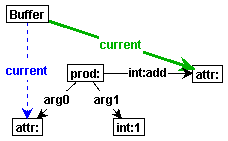
\includegraphics{\figdir/update}
\flabel{update}
}
\subfigure[Output]{
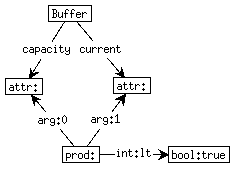
\includegraphics{\figdir/condition}
\flabel{condition}
}
\caption{Using attribute values.}
\flabel{attribute-usage}
\end{center}
\end{figure}

\subsection{Editor format}
\stlabel{input}

The visual formatting of attributed graphs, production rules, and
labelled transition systems, described in the previous section, is the
\emph{display format}. In the editor of the GROOVE tool and for the
purpose of serialising and exchanging production rules, we need a
textual representation of this format. This is true for all of them.

\subsubsection{Attributed graphs}

\fref{algebra-buffer-state} shows the display format of the attributed
graph as well as the editor format. From that figure we want to
address how to include constant data values from different data
types. The general rule is to encode data values as labels of
self-edges of the node representing the data value. These labels are
then of the form: \prefix:\constantSymbol, where \prefix{} must be
replaced by one of the prefixes listed in \tref{data-types} and
\constantSymbol{} by a textual representation of the actual data
value.\footnote{In the GXL format the self-edge of nodes representing
  data values is stored as a simple edge with the entire label. In the
  near future we plan to use GXL-specific encodings for this in order
  to make the graph exported by GROOVE easier to process by other
  tools.} Some examples are given in \tref{algebra-values}.

\begin{table}[htbp]
  \centering
  \begin{tabular}{|c|c|}
  \hline\hline
  {\bf Data Type} & {\bf Prefix} \\
  \hline
  Integer & \texttt{int} \\
  String & \texttt{string} \\
  Boolean & \texttt{bool} \\
  \hline\hline
  \end{tabular}
  \caption{Data types with their corresponding prefixes.}
  \tlabel{data-types}
\end{table}

\begin{table}[htbp]
  \centering
  \begin{tabular}{|c|c|}
  \hline\hline
  {\bf Data Value} & {\bf Editor Format} \\
  \hline
  integer 1 & \texttt{int:1} \\
  string ``hello'' & \texttt{string:hello} \\
  boolean \true & \texttt{bool:true} \\
  \hline\hline
  \end{tabular}
  \caption{Data values with their corresponding editor format.}
  \tlabel{algebra-values}
\end{table}

\subsubsection{Production rules}

In particular, we need a way to categorise rule
nodes and edges as reader, eraser, embargo or creator. This is done by
introducing special \emph{role prefixes}, listed in \tref{prefixes}.
%
\begin{table}[htbp]
\begin{center}
\begin{tabular}{|c|l|}
\hline\hline
\bf Prefix & \bf Meaning \\
\hline
\emph{(none)} & Reader node or edge \\
\Use & Reader node or edge \\
\Del & Eraser node or edge \\
\Not & Embargo node or edge (incl.\ merge embargo) \\
\New & Creator node or edge (incl.\ merger) \\
\hline
\Start & Start node of a labelled transition system \\
\Final & Final node of a labelled transition system \\
\Open & Open node of a labelled transition system \\
\hline\hline
\end{tabular}
\end{center}
\caption{Role prefixes in the editor format for production rules and labelled
transition systems.}
\tlabel{prefixes}
\end{table}
%
For nodes, the role is indicated by a special self-edge labeled exclusively by
the role prefix; for edges, the prefix is inserted in front of the edge label.
Note that reader elements do not necessarily need a role prefix: the absence of
any prefix indicates a reader node or edge. Furthermore, for edges incident to
eraser, embargo or creator nodes the role prefix can be left out, since it is
implicit.
%
\texfig{rule-input}{
    The rules of Figures~\ref{f:append-rule} and \ref{f:assign-rule} in editor
    format.
}%
%
As an example, \fref{rule-input} shows the production rules of
Figures~\ref{f:append-rule} and \ref{f:assign-rule} in editor format.
\fref{circular-input} shows the editor format of the rules in
\fref{circular-display}.
%
\texfig{circular-input}{The production rules \Put{} and \Get{} of
  \fref{circular-display} in editor format.}

When specifying production rules over attributed graphs, we need to
introduce a way to refer to algebraic operations to be applied on
particular data values. Since we cannot assume that every operation
(no matter from which data type) has a distinct symbol, we need an
editor format comparable to the one used for data values:
\prefix:\operationSymbol, where \operationSymbol{} must be replaced by
the textual representations of the specific algebraic operation, as
listed in \tref{algebra-operations}.

\begin{table}[htbp]
  \centering
  \begin{tabular}{|c|c|c|}
  \hline\hline
  {\bf Data Type} & {\bf Operation Symbol} & {\bf Editor Format} \\
  \hline
  \multirow{8}*{Integer} & $+$  & \texttt{add} \\
                         & $-$  & \texttt{sub} \\
                         & $*$  & \texttt{mul} \\
                         & $/$  & \texttt{div} \\
                         & $\%$ & \texttt{mod} \\
                         & $=$  & \texttt{eq} \\
                         & $<$  & \texttt{lt} \\
                         & $<=$  & \texttt{le} \\
                         & $>$  & \texttt{gt} \\
                         & $>=$  & \texttt{ge} \\
  \hline
  \multirow{2}*{String}  & $+$  & \texttt{concat} \\
                         & $=$  & \texttt{eq} \\
  \hline
  \multirow{2}*{Boolean} & $\wedge$ & \texttt{and} \\
                         & $\vee$   & \texttt{or} \\
                         & $\neg$   & \texttt{not} \\
  \hline\hline
  \end{tabular}
  \caption{Algebraic operations with their corresponding editor format.}
  \tlabel{algebra-operations}
\end{table}

\fref{algebra-buffer-transformation-input} shows the editor format of
the production rule from \fref{algebra-buffer-transformation-output}.

\texfig{algebra-buffer-transformation-input}{Editor format of the
  production rule from \fref{algebra-buffer-transformation-output}.}

\subsubsection{Labelled transition systems}

Although labelled transition systems are not created in the editor but during
simulation of a production system, they can be saved as graphs and subsequently
edited or otherwise processed. In this case, some of the visual elements in the
display of labelled transition systems, discussed above, are also encoded
through special labels. This happens for the initial, final and open
states; however, information about the active state or transition is
lost, as are the state identifiers.

The spedial labels used for this purpose are also listed in
\tref{prefixes}. \fref{lts-graphs} shows the editor format of the two
transition systems of \fref{ltss}.

\texfig{lts-graphs}{The labelled transition systems of \fref{ltss} in editor format.}


%%% Local Variables: 
%%% mode: latex
%%% TeX-master: "usermanual"
%%% End: 
